\documentclass[12pt,a4paper]{article}

% ─── Page Layout ───────────────────────────────────────────────────────────────
\usepackage[a4paper, margin=0.8in, headheight=14pt]{geometry}

% ─── Fonts (XeLaTeX) ───────────────────────────────────────────────────────────
\usepackage{fontspec}
\usepackage{unicode-math}
\setmainfont{TeX Gyre Pagella}
\setmonofont[Scale=0.88]{TeX Gyre Cursor}
\setmathfont{Latin Modern Math}

% ─── Packages ──────────────────────────────────────────────────────────────────
\usepackage{xcolor}
\usepackage{colortbl}
\usepackage{titlesec}
\usepackage{enumitem}
\usepackage{tabularx}
\usepackage{booktabs}
\usepackage{array}
\usepackage{amsmath}
\usepackage{tikz}
\usetikzlibrary{shapes.geometric, arrows.meta, positioning, calc, fit, decorations.pathreplacing}
\usepackage{tcolorbox}
\tcbuselibrary{skins, breakable}
\usepackage{hyperref}
\usepackage{fancyhdr}
\usepackage{graphicx}
\usepackage{microtype}
\hyphenpenalty=10000
\exhyphenpenalty=10000
\sloppy
\usepackage{caption}
\usepackage{setspace}
\usepackage{multirow}
\usepackage{tocloft}

% ─── Q&A helper ────────────────────────────────────────────────────────────────
\newcommand{\Q}[1]{\textbf{#1}\par\noindent\ignorespaces}

% ─── Colour Palette ────────────────────────────────────────────────────────────
\definecolor{myred}{RGB}{196,30,58}
\definecolor{mydark}{RGB}{30,30,50}
\definecolor{mygreen}{RGB}{14,120,80}
\definecolor{myteal}{RGB}{0,130,140}
\definecolor{myamber}{RGB}{180,100,0}
\definecolor{mypurple}{RGB}{100,30,160}
\definecolor{mygray}{RGB}{246,247,249}
\definecolor{mgframe}{RGB}{180,185,200}
\definecolor{watermark}{RGB}{145,150,170}
\definecolor{hdrred}{RGB}{250,232,235}
\definecolor{hdrgreen}{RGB}{220,244,233}
\definecolor{hdrteal}{RGB}{220,242,244}
\definecolor{hdramber}{RGB}{253,242,215}
\definecolor{hdrpurple}{RGB}{238,228,255}
\definecolor{hdrgray}{RGB}{238,240,245}
\definecolor{rowalt}{RGB}{250,251,253}

% ─── Section Formatting ────────────────────────────────────────────────────────
\titleformat{\section}
  {\large\bfseries\color{myred}}{\thesection.}{0.5em}{}
  [\vspace{1pt}{\color{myred}\rule{\linewidth}{0.8pt}}]
\titleformat{\subsection}
  {\normalsize\bfseries\color{myteal}}{\thesubsection}{0.5em}{}
\titlespacing*{\section}{0pt}{18pt}{7pt}
\titlespacing*{\subsection}{0pt}{11pt}{4pt}

% ─── Paragraph ─────────────────────────────────────────────────────────────────
\setlength{\parindent}{0pt}
\setlength{\parskip}{4pt}

% ─── TOC Styling ───────────────────────────────────────────────────────────────
\renewcommand{\cfttoctitlefont}{\large\bfseries\color{myred}}
\renewcommand{\cftaftertoctitle}{\par\noindent{\color{myred}\rule{\linewidth}{0.8pt}}}
\setlength{\cftbeforetoctitleskip}{0pt}
\setlength{\cftaftertoctitleskip}{6pt}
\renewcommand{\cftsecfont}{\normalsize\bfseries\color{mydark}}
\renewcommand{\cftsecpagefont}{\normalsize\bfseries\color{mydark}}
\renewcommand{\cftsecleader}{\cftdotfill{\cftdotsep}}
\setlength{\cftbeforesecskip}{7pt}
\renewcommand{\cftsubsecfont}{\small\color{mydark}}
\renewcommand{\cftsubsecpagefont}{\small\color{mydark}}
\setlength{\cftbeforesubsecskip}{3pt}
\setlength{\cftsubsecindent}{1.4em}

% ─── Table helpers ─────────────────────────────────────────────────────────────
\renewcommand{\arraystretch}{1.45}
\setlength{\tabcolsep}{6pt}
\arrayrulecolor{mydark}
\newcolumntype{B}[1]{>{\small\bfseries\raggedright\arraybackslash}m{#1}}
\newcolumntype{Y}{>{\small\raggedright\arraybackslash}X}
\renewcommand{\tabularxcolumn}[1]{m{#1}}

% ─── Header / Footer ───────────────────────────────────────────────────────────
\pagestyle{fancy}
\fancyhf{}
\fancyhead[L]{\small\color{myred}\textbf{EC501}\;\color{mydark}--- Electromagnetic Waves}
\fancyhead[R]{\small\color{myteal}\textbf{Module 2 Notes}}
\fancyfoot[C]{\small\color{mydark}\thepage}
\fancyfoot[R]{\small\color{watermark}\textit{\copyright\ Biraj}}
\renewcommand{\headrulewidth}{0.5pt}
\renewcommand{\footrulewidth}{0.3pt}

% ─── Hyperref ──────────────────────────────────────────────────────────────────
\hypersetup{
  colorlinks=true, linkcolor=myteal, urlcolor=myteal,
  pdfauthor={Biraj Sarkar},
  pdftitle={EC501 --- Module 2 Notes}
}

% ─── tcolorbox styles ──────────────────────────────────────────────────────────
\tcbset{
  tikzbox/.style={
    colback=mygray, colframe=mgframe, boxrule=0.6pt, arc=4pt,
    left=8pt, right=8pt, top=6pt, bottom=6pt,
    colbacktitle=mgframe, coltitle=mydark,
    fonttitle=\small\bfseries
  },
  defbox/.style={
    colback=hdrgreen, colframe=mygreen, boxrule=0.8pt, arc=4pt,
    left=9pt, right=9pt, top=6pt, bottom=6pt,
    colbacktitle=mygreen, coltitle=white,
    fonttitle=\small\bfseries
  },
  formulabox/.style={
    colback=hdrteal, colframe=myteal, boxrule=0.8pt, arc=4pt,
    left=9pt, right=9pt, top=7pt, bottom=7pt,
    colbacktitle=myteal, coltitle=white,
    fonttitle=\small\bfseries
  },
  examplebox/.style={
    colback=hdramber, colframe=myamber, boxrule=0.8pt, arc=4pt,
    left=9pt, right=9pt, top=6pt, bottom=6pt,
    colbacktitle=myamber, coltitle=white,
    fonttitle=\small\bfseries
  },
  masonbox/.style={
    colback=hdrpurple, colframe=mypurple, boxrule=0.8pt, arc=4pt,
    left=9pt, right=9pt, top=6pt, bottom=6pt,
    colbacktitle=mypurple, coltitle=white,
    fonttitle=\small\bfseries
  },
  exambox/.style={
    colback=hdrpurple, colframe=mypurple, boxrule=1pt, arc=5pt,
    left=10pt, right=10pt, top=8pt, bottom=8pt,
    colbacktitle=mypurple, coltitle=white,
    fonttitle=\bfseries,
    breakable, title after break={\textbf{Frequently Asked / Viva Questions (contd.)}}}
}
% Make all boxes breakable across pages
\tcbset{breakable}

% ─── TikZ styles ───────────────────────────────────────────────────────────────
\tikzset{
  block/.style={rectangle, draw=myteal, fill=hdrteal,
    text width=2.4cm, align=center, minimum height=0.95cm,
    font=\small, rounded corners=3pt, line width=0.7pt},
  redblock/.style={rectangle, draw=myred, fill=hdrred,
    text width=2.4cm, align=center, minimum height=0.95cm,
    font=\small, rounded corners=3pt, line width=0.7pt},
  netnode/.style={rectangle, draw=myteal, fill=hdrteal,
    text width=1.5cm, align=center, minimum height=0.8cm,
    font=\small, rounded corners=3pt, line width=0.7pt},
  sumjunc/.style={circle, draw=myamber, fill=hdramber,
    minimum size=0.62cm, font=\small, line width=0.8pt},
  snode/.style={circle, draw=mypurple, fill=hdrpurple,
    minimum size=0.55cm, font=\footnotesize, line width=0.7pt},
  arrow/.style={-Stealth, thick, color=mydark},
  redarrow/.style={-Stealth, thick, color=myred},
  line/.style={thick, color=mydark}
}

% ═══════════════════════════════════════════════════════════════════════════════
\begin{document}
% ═══════════════════════════════════════════════════════════════════════════════

\begin{center}
  {\LARGE\bfseries\color{myred} EC501 --- Electromagnetic Waves}\\[5pt]
  {\normalsize\color{mydark} Semester V \quad$\bullet$\quad 3L:0T:0P \quad$\bullet$\quad 3 Credits}\\[3pt]
  {\normalsize\color{myteal}\textbf{Module 2 Exam Notes: Uniform Plane Waves and Media Interfaces}}\\[3pt]
  {\small\color{mydark} CGEC \;$|$\; B.Tech ECE (2023--27) \;$|$\; \textit{Biraj Sarkar}}
\end{center}
\vspace{2pt}
\noindent{\color{myred}\rule{\linewidth}{1.5pt}}
\vspace{2pt}

\hypersetup{linkcolor=mydark}
\tableofcontents
\hypersetup{linkcolor=myteal}
\newpage

\section{Uniform Plane Waves}
\begin{tcolorbox}[defbox,title={Uniform plane wave}]
A uniform plane wave has the same field at every point in a plane perpendicular to propagation. In a source-free homogeneous isotropic medium the electric and magnetic fields are transverse.
\end{tcolorbox}
\subsection{Wave equation and travelling fields}
Use peak phasors with $e^{j\omega t}$ and real material constants $\mu,\epsilon,\sigma$. In a source-free bulk medium, $\nabla\cdot\mathbf E=0$. Taking curl of Faraday's law gives
\[
\begin{aligned}
\nabla\times\nabla\times\mathbf E
 &=-j\omega\mu(\sigma+j\omega\epsilon)\mathbf E,\\
\nabla^2\mathbf E&=\gamma^2\mathbf E,\qquad
\gamma=\sqrt{j\omega\mu(\sigma+j\omega\epsilon)}=\alpha+j\beta .
\end{aligned}
\]
Curling Amp\`ere--Maxwell in the same homogeneous medium gives $\nabla^2\mathbf H=\gamma^2\mathbf H$ using $\nabla\cdot\mathbf H=0$. In time domain the electric-field equation is
\[
 \nabla^2\mathbf E=\mu\sigma\,\partial_t\mathbf E+
                      \mu\epsilon\,\partial_t^2\mathbf E.
\]
The first term accounts for conduction and the second for displacement current.
The decaying forward solution is $\mathbf E=\mathbf E_0e^{-\gamma\hat{\mathbf k}\cdot\mathbf r}$. Use $\nabla\times\mathbf E=-\gamma\hat{\mathbf k}\times\mathbf E$ to obtain $\mathbf H=\hat{\mathbf k}\times\mathbf E/\eta$, where $\eta=j\omega\mu/\gamma$ in ohms.
\begin{itemize}[leftmargin=*,itemsep=3pt]
\item \textbf{Lossless limit.} $\alpha=0$, $\beta=k=\omega\sqrt{\mu\epsilon}$ and $\eta=\sqrt{\mu/\epsilon}$. In free space $v=1/\sqrt{\mu_0\epsilon_0}\approx 3\times10^8\,\mathrm{m/s}$ and $\eta_0\approx377\,\Omega$.
\item \textbf{Phase velocity.} Keeping $\omega t-\beta z$ constant gives $v_p=\omega/\beta=f\lambda$. Here $\lambda=2\pi/\beta$.
\item \textbf{Group velocity.} Superpose nearby frequencies and write the envelope phase as $\Delta\omega\,t-\Delta\beta\,z$. The envelope moves at $v_g=d\omega/d\beta$ for a narrow band with weak distortion. For $\beta$ proportional to $\omega$, $v_g=v_p$. With strong loss or dispersion, a reshaped pulse peak need not track energy.
\end{itemize}

\subsection{Polarization and the Poincar\'e sphere}
\begin{tcolorbox}[defbox,title={Polarization}]
Polarization describes the trajectory and sense traced by the tip of the electric field at a fixed point. Only the relative amplitudes and phases of the transverse components matter.
\end{tcolorbox}

For propagation along $+z$, use $\mathbf E=(a\hat{\mathbf x}+be^{j\Delta}\hat{\mathbf y})e^{-jkz}$ with $a,b\ge0$. At fixed $z$ write $u=E_x/a$ and $v=E_y/b$. Eliminating the common time phase from $u=\cos\psi$ and $v=\cos(\psi+\Delta)$ gives
\[
u^2+v^2-2uv\cos\Delta=\sin^2\Delta .
\]
\begin{itemize}[leftmargin=*,itemsep=3pt]
\item \textbf{Linear.} Relative phase $0$ or $\pi$, or one component zero. The field moves along a fixed line.
\item \textbf{Circular.} Equal magnitudes and $\Delta=\pm\pi/2$. For $\Delta=-\pi/2$ the field initially moves from $+x$ towards $+y$. State the viewing direction if giving a handedness name.
\item \textbf{Elliptical.} The general nondegenerate case. Axial ratio is major semiaxis divided by minor semiaxis, so it equals 1 for a circle and tends to infinity for a line.
\end{itemize}
For a fully polarized wave, the normalized Stokes coordinates $s_i=S_i/S_0$ give a point on the unit Poincar\'e sphere:
\[
\begin{aligned}
S_0 &= a^2+b^2,&S_1 &=a^2-b^2,\\
S_2 &=2ab\cos\Delta,& S_3 &=2ab\sin\Delta .
\end{aligned}
\]
This choice defines the pole signs. Verify $S_1^2+S_2^2+S_3^2=S_0^2$ by squaring. The ellipse tilt is $\tfrac12\operatorname{atan2}(s_2,s_1)$ and signed ellipticity angle is $\chi=\tfrac12\sin^{-1}(s_3)$. The axial ratio is $1/|\tan\chi|$. At the poles the tilt is undefined. The equator is linear, poles are circular, and antipodal points represent orthogonal states.
\begin{tcolorbox}[tikzbox,title={Poincar\'e sphere for the stated Stokes convention},unbreakable]
\centering
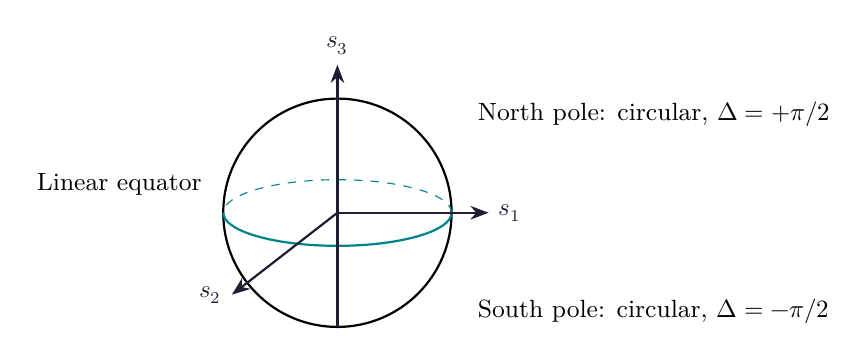
\begin{tikzpicture}[font=\small]
\draw[thick] (0,0) circle (1.45);
\draw[dashed,myteal] (1.45,0) arc (0:180:1.45 and .42);
\draw[myteal,thick] (-1.45,0) arc (180:360:1.45 and .42);
\draw[arrow] (0,-1.45)--(0,1.88) node[above] {$s_3$};
\draw[arrow] (0,0)--(1.92,0) node[right] {$s_1$};
\draw[arrow] (0,0)--(-1.34,-1.04) node[left] {$s_2$};
\node[anchor=west] at (1.66,1.25) {North pole: circular, $\Delta=+\pi/2$};
\node[anchor=west] at (1.66,-1.25) {South pole: circular, $\Delta=-\pi/2$};
\node[anchor=east] at (-1.6,.36) {Linear equator};
\end{tikzpicture}
\end{tcolorbox}

For $(E_x,E_y)=(3,-j)\,\mathrm{V/m}$, the axes are $x,y$ and axial ratio is 3. The normalized point is $(8/10,0,-6/10)$.

\section{Propagation in Conducting Media}
\begin{tcolorbox}[defbox,title={Skin depth}]
Skin depth $\delta=1/\alpha$ is the distance over which a plane-wave field amplitude falls to $1/e$ of its surface value.
\end{tcolorbox}

Squaring $\gamma=\alpha+j\beta$ gives $\beta^2-\alpha^2=\omega^2\mu\epsilon$ and $2\alpha\beta=\omega\mu\sigma$. Squaring and adding gives $\beta^2+\alpha^2=\omega^2\mu\epsilon\sqrt{1+(\sigma/\omega\epsilon)^2}$. Thus, with $t=\sigma/(\omega\epsilon)$,
\[
\alpha=\omega\sqrt{\frac{\mu\epsilon}{2}(\sqrt{1+t^2}-1)},\qquad
\beta=\omega\sqrt{\frac{\mu\epsilon}{2}(\sqrt{1+t^2}+1)} .
\]
\begin{itemize}[leftmargin=*,itemsep=3pt]
\item \textbf{Low-loss dielectric} ($t\ll1$). $\beta\approx\omega\sqrt{\mu\epsilon}$ and $\alpha\approx(\sigma/2)\sqrt{\mu/\epsilon}$.
\item \textbf{Good conductor} ($t\gg1$). $\gamma\approx(1+j)\sqrt{\omega\mu\sigma/2}$, $\delta\approx\sqrt{2/(\omega\mu\sigma)}$ and $\eta\approx(1+j)R_s$ where $R_s=1/(\sigma\delta)$ in $\Omega$ per square.
\item \textbf{Current and power.} For a thick, locally flat conductor, inward depth $u$ gives $\mathbf J_t(u)=\sigma\mathbf E_t(0)e^{-(1+j)u/\delta}$. Integrating gives equivalent sheet current $\mathbf K=\sigma\mathbf E_t(0)/\gamma$. The metal-to-outside normal gives $\mathbf K\approx\hat{\mathbf n}\times\mathbf H_t$.
\end{itemize}
The ratio $t$ compares the magnitudes of conduction and displacement current densities. A perfect dielectric has $t=0$. A lossy dielectric has nonzero conductivity in this model, and the low-loss approximation requires $t\ll1$. Around $t=1$ use both terms. For instance, a material with $\epsilon_r=12$ and $\sigma=0.001\,\mathrm{S/m}$ has $t\approx0.30$ at $5\,\mathrm{MHz}$. With $\epsilon_r=60$ and $\sigma=1.2\,\mathrm{S/m}$ at the same frequency, $t\approx72$ and the good-conductor approximation is appropriate.

With peak phasors, the mean loss per unit area is
\[
\begin{aligned}
p_s&=\int_0^\infty \tfrac12\sigma|\mathbf E_t(0)|^2 e^{-2u/\delta}\,du\\
   &=\frac{\sigma\delta}{4}|\mathbf E_t(0)|^2
    =\tfrac12 R_s |\mathbf H_t(0)|^2 .
\end{aligned}
\]
\begin{tcolorbox}[examplebox,title={Skin depth and heating in copper}]
At $10\,\mathrm{MHz}$ take $\mu=\mu_0$ and $\sigma=5.8\times10^7\,\mathrm{S/m}$. Then $\delta\approx20.9\,\mu\mathrm m$ and $R_s\approx0.825\,\mathrm{m}\Omega$. At $|\mathbf H_t|=10\,\mathrm{A/m}$ peak, $p_s\approx0.0413\,\mathrm{W/m^2}$.
\end{tcolorbox}

\begin{tcolorbox}[examplebox,title={Extract wave parameters from attenuation data}]
At $20\,\mathrm{MHz}$ a wave has $\beta=2.4\,\mathrm{rad/m}$ and retains $25\%$ of its field amplitude after $3\,\mathrm m$. Use $|E(z)|/|E(0)|=e^{-\alpha z}$.
\[
\begin{aligned}
 \alpha&=-\ln(0.25)/3=0.462\,\mathrm{Np/m},\\
 \delta&=1/\alpha=2.16\,\mathrm m,\\
 v_p&=2\pi f/\beta=5.24\times10^7\,\mathrm{m/s}.
\end{aligned}
\]
For this uniform forward wave the power fraction is $e^{-2\alpha z}$. A statement that $25\%$ of the \emph{power} remains would give half the above attenuation constant.
\end{tcolorbox}

\section{Plane Waves at a Media Interface}
\subsection{Arbitrary direction, reflection and refraction}
At $z=0$ take incidence from medium 1 ($z<0$) into medium 2. Rotate the axes so the plane of incidence is $xz$. An arbitrary incident direction then has $\mathbf k_i=k_1(\hat{\mathbf x}\sin\theta_i+\hat{\mathbf z}\cos\theta_i)$ and a phase factor $e^{-j\mathbf k_i\cdot\mathbf r}$ in a lossless medium. Tangential phase factors must match at every point on the interface. Therefore
\[
 k_1\sin\theta_i=k_1\sin\theta_r=k_2\sin\theta_t .
\]
This gives $\theta_r=\theta_i$ and Snell's law. For isotropic dielectrics use $n_1\sin\theta_i=n_2\sin\theta_t$, where $n_m=ck_m/\omega$.
\begin{tcolorbox}[tikzbox,title={Oblique incidence and tangential phase matching},unbreakable]
\centering
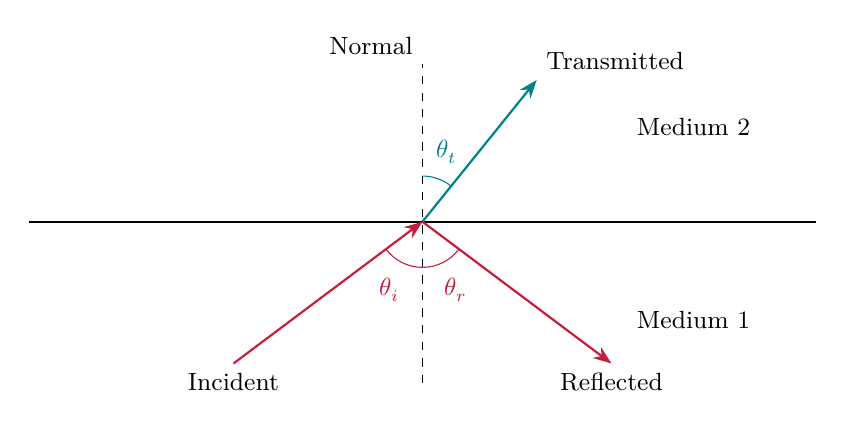
\begin{tikzpicture}[font=\small]
\draw[thick] (-5,0)--(5,0);
\draw[dashed] (0,-2.05)--(0,2.0) node[above left] {Normal};
\draw[redarrow] (-2.4,-1.8)--(0,0);
\draw[redarrow] (0,0)--(2.4,-1.8);
\draw[arrow,color=myteal] (0,0)--(1.45,1.8);
\node[anchor=west] at (2.6,1.2) {Medium 2};
\node[anchor=west] at (2.6,-1.25) {Medium 1};
\node[below] at (-2.4,-1.8) {Incident};
\node[below] at (2.4,-1.8) {Reflected};
\node[above right] at (1.45,1.8) {Transmitted};
\draw[myred] (0,-.58) arc[start angle=270,end angle=217,radius=.58];
\draw[myred] (0,-.58) arc[start angle=270,end angle=323,radius=.58];
\draw[myteal] (0,.58) arc[start angle=90,end angle=51,radius=.58];
\node[myred] at (-.42,-.86) {$\theta_i$};
\node[myred] at (.42,-.86) {$\theta_r$};
\node[myteal] at (.31,.89) {$\theta_t$};
\end{tikzpicture}
\end{tcolorbox}
\subsection{TE, TM and Fresnel coefficients}
Transverse electric (TE or s) has $\mathbf E$ perpendicular to the incidence plane. Transverse magnetic (TM or p) has $\mathbf H$ perpendicular to that plane. Define $E_i,E_r,E_t$ as signed \emph{tangential electric} components along the same coordinate direction in all three waves. For one forward component the wave admittance is $Y_{\mathrm{TE}}=\cos\theta/\eta$ and $Y_{\mathrm{TM}}=1/(\eta\cos\theta)$, obtained by resolving $\mathbf H=\hat{\mathbf k}\times\mathbf E/\eta$.
\[
\begin{aligned}
E_i+E_r &= E_t,&
Y_1(E_i-E_r)&=Y_2E_t,\\
r=\frac{E_r}{E_i}&=\frac{Y_1-Y_2}{Y_1+Y_2},&
t_E=\frac{E_t}{E_i}&=1+r=\frac{2Y_1}{Y_1+Y_2}.
\end{aligned}
\]
\begin{itemize}[leftmargin=*,itemsep=3pt]
\item \textbf{Normal incidence.} Both polarizations give $r=(\eta_2-\eta_1)/(\eta_1+\eta_2)$. At oblique incidence $t_E$ for TM refers to tangential components, so the total field ratio adds a factor $\cos\theta_i/\cos\theta_t$.
\item \textbf{Power ratios.} The normal flux is $\tfrac12\operatorname{Re}(Y)|E_{\tan}|^2$ for a forward wave. For a lossless incident medium, $R=|r|^2$ and $T=\operatorname{Re}(Y_2)|t_E|^2/Y_1$. At an ordinary lossless interface $R+T=1$.
\item \textbf{Brewster angle.} For equal permeabilities and different real refractive indices, TM reflection vanishes when $Y_{1,\mathrm{TM}}=Y_{2,\mathrm{TM}}$. Substituting $\eta_m\propto1/n_m$ and Snell's law gives $\theta_i+\theta_t=90^\circ$, hence $\tan\theta_B=n_2/n_1$. Reflected light can therefore be purely TE.
\item \textbf{Polarization change.} Decompose the incident field into TE and TM and apply each coefficient separately. Unequal magnitudes alter the orientation and axial ratio. A relative phase change, such as in total internal reflection, can turn linear polarization into elliptical.
\end{itemize}
\begin{tcolorbox}[examplebox,title={Compare TE and TM power reflection at oblique incidence}]
From air onto a lossless nonmagnetic dielectric with $n_2=2$, let $\theta_i=30^\circ$. Snell gives $\sin\theta_t=0.25$ and $\cos\theta_t=0.9682$. Use $\eta_2=\eta_0/2$.
\[
\begin{aligned}
 r_{\mathrm{TE}}&=\frac{0.8660-1.9365}{0.8660+1.9365}
                  =-0.382,& R_{\mathrm{TE}}&=0.146,\\
 r_{\mathrm{TM}}&=\frac{1.1547-2.0656}{1.1547+2.0656}
                  =-0.283,& R_{\mathrm{TM}}&=0.080.
\end{aligned}
\]
The numerators use the tangential-electric convention and both admittances are scaled by $\eta_0$. Power transmittance is $1-R$ for each polarization. The negative field sign gives phase reversal, not negative reflected power.
\end{tcolorbox}

\subsection{Total internal reflection and conducting boundary}
For $n_1>n_2$ the critical angle is $\theta_c=\sin^{-1}(n_2/n_1)$. Above it $k_x>k_2$ and $k_{2z}=-j\kappa$ with $\kappa=\sqrt{k_x^2-k_2^2}$ for decay into $z>0$. The transmitted field varies as $e^{-jk_x x}e^{-\kappa z}$. It is evanescent and has zero mean normal power in a lossless second half-space. The reflected magnitude is unity but its phase can differ between TE and TM.
\begin{tcolorbox}[examplebox,title={Glass to air and air to glass}]
Glass-to-air with $n_1=1.5$, $n_2=1$ gives $\theta_c=\sin^{-1}(1/1.5)=41.8^\circ$. At $50^\circ$, $k_x=1.149k_0$ and $\kappa=0.566k_0$. In the reverse direction at normal incidence, $r=(377/1.5-377)/(377/1.5+377)=-0.2$. Power reflection is $4\%$ and transmission is $96\%$.
\end{tcolorbox}

For a perfect electric conductor, $\mathbf E_{\tan}=0$ so $r=-1$ for tangential electric field. At normal incidence onto $z=0$ from $z<0$,
\[
 E_x=-2jE_0\sin(kz),\qquad H_y=2(E_0/\eta)\cos(kz).
\]
The wall is an electric node and a magnetic antinode, and mean normal power is zero. For a finite good conductor, use its complex $\eta$ at normal incidence. The reflected amplitude is below unity and the transmitted normal power is dissipated over the skin layer.
At oblique PEC incidence the reflected tangential electric component again has opposite sign. Let $\psi=e^{-jk_x x}$ and let $E_i$ be the tangential electric amplitude at the wall reference plane. Then $E_{\tan}=-2j E_i\psi\sin(k_z z)$. For TE this is the entire electric field. For TM use $\mathbf k\cdot\mathbf E=0$ separately for each wave to get $E_z=-2(k_x/k_z) E_i\psi\cos(k_z z)$. Normal electric field at the wall is allowed and is supported by surface charge. The tangential magnetic fields add at the wall and support surface current.

\newpage
\begin{center}
  {\large\bfseries\color{myred} Quick Revision --- Module 2}\\[3pt]
  {\small\color{mydark} Uniform Plane Waves and Media Interfaces $|$ EC501}
\end{center}
\noindent{\color{myred}\rule{\linewidth}{1.2pt}}
\begin{tcolorbox}[formulabox,title={Key Formulas at a Glance}]
\renewcommand{\arraystretch}{1.35}
\begin{tabularx}{\linewidth}{B{5.0cm}Y}
Propagation & $\gamma^2=j\omega\mu(\sigma+j\omega\epsilon)$ \\[3pt]
Speed & $v_p=\omega/\beta$, $v_g=d\omega/d\beta$ \\[3pt]
Skin depth & $\delta=1/\alpha\approx\sqrt{2/(\omega\mu\sigma)}$ in a good conductor \\[3pt]
Phase matching & $n_1\sin\theta_i=n_2\sin\theta_t$ \\[3pt]
Fresnel coefficient & $r=(Y_1-Y_2)/(Y_1+Y_2)$ for tangential electric field \\[3pt]
Total internal reflection & $\theta_c=\sin^{-1}(n_2/n_1)$ for $n_1>n_2$ \\[3pt]
\end{tabularx}
\end{tcolorbox}
\begin{tcolorbox}[defbox,title={One-Line Definitions}]
\textbf{Wave impedance.} Ratio of transverse electric to magnetic magnitudes as a complex field ratio, in ohms.\par
\textbf{Polarization.} Locus and rotation sense of the electric vector at a fixed point.\par
\textbf{Evanescent field.} A field whose amplitude decays exponentially in a spatial direction.\par
\end{tcolorbox}
\begin{tcolorbox}[exambox,title={Frequently Asked / Viva Questions}]
\begin{enumerate}[topsep=0pt, label=\textbf{Q\arabic*.}, itemsep=5pt]
\item \Q{What is uniform on a plane-wave wavefront?}
The field across a plane normal to propagation.
\item \Q{When is a transverse wave circular?}
Equal orthogonal amplitudes in phase quadrature.
\item \Q{What is plotted on the Poincar\'e sphere?}
The three normalized Stokes coordinates.
\item \Q{What distinguishes phase and group velocity?}
One follows a phase point and the other follows a narrow-band envelope.
\item \Q{Why does copper carry high-frequency current near its surface?}
Its high conductivity gives a large attenuation constant and small skin depth.
\item \Q{What is the surface-loss density for a peak field?}
$\tfrac12R_s|\mathbf H_t|^2$.
\item \Q{Why must tangential wave number match?}
The boundary conditions must hold at all points of the interface.
\item \Q{Which dielectric reflection vanishes at Brewster incidence?}
TM for lossless dielectrics of equal permeability.
\item \Q{What remains in the second medium above the critical angle?}
A decaying field with zero mean normal flux in a lossless half-space.
\item \Q{What is the PEC electric reflection coefficient?}
Minus one for the tangential electric component.
\end{enumerate}
\end{tcolorbox}
\begin{tcolorbox}[tikzbox,title={Summary comparison}]
\begin{tabularx}{\linewidth}{|B{4cm}|Y|}\hline
\textbf{Case} & \textbf{What to use} \\ \hline
Lossless plane wave & Real $\eta$ and no attenuation. \\ \hline
Good conductor & $\alpha\approx\beta$, with $\eta\approx(1+j)R_s$. \\ \hline
TE / TM & $Y=\cos\theta/\eta$ for TE, $Y=1/(\eta\cos\theta)$ for TM. \\ \hline
\end{tabularx}
\end{tcolorbox}
\end{document}
